% IE 643 Project Report -- Team Gradient Mavericks
% Built from the official IE643_2026_Report_template (header macro, margins and section structure kept).
% Compile:  tectonic IE643_Project_Report.tex   (or pdflatex + bibtex + pdflatex x2)

\documentclass[twoside,english]{article}
\setlength{\oddsidemargin}{0.25 in}
\setlength{\evensidemargin}{-0.25 in}
\setlength{\topmargin}{-0.6 in}
\setlength{\textwidth}{6.5 in}
\setlength{\textheight}{8.5 in}
\setlength{\headsep}{0.75 in}
\setlength{\parindent}{0 in}
\setlength{\parskip}{0.1 in}

%
% ADD PACKAGES here:
%
\usepackage{amsmath,amsfonts,amssymb,graphicx,algorithm,caption}
\usepackage[noend]{algpseudocode}
\usepackage{hyperref}
\usepackage{natbib}
\usepackage[document]{ragged2e}
\usepackage{mathtools}
\usepackage{xcolor}
\usepackage{booktabs}
\usepackage{multirow}
\usepackage{tikz}
\usetikzlibrary{arrows.meta,positioning,fit,backgrounds,calc}
\hypersetup{colorlinks=true,linkcolor=blue!50!black,citecolor=blue!50!black,urlcolor=blue!50!black}

\newcounter{lecnum}
\renewcommand{\thepage}{\arabic{page}}
\renewcommand{\thesection}{\arabic{section}}
\renewcommand{\theequation}{\arabic{equation}}
\renewcommand{\thefigure}{\arabic{figure}}
\renewcommand{\thetable}{\arabic{table}}
\makeatletter
\def\BState{\State\hskip-\ALG@thistlm}
\makeatother

\newcommand{\lecture}[4]{
   \pagestyle{myheadings}
   \thispagestyle{plain}
   \newpage
   \setcounter{page}{1}
   \noindent
   \begin{center}
   \framebox{
      \vbox{\vspace{2mm}
    \hbox to 6.28in { {\bf IE 643: Deep Learning - Theory and Practice
		\hfill July-Dec 2026} }
       \vspace{4mm}
       \hbox to 6.28in {\parbox{6.28in}{\centering\large Project Report: #1}}
       \vspace{2mm}
       \vspace{2mm}
       \hbox to 6.28in { {\it Team Name: #2 \hfill Team Members: #3} }
      \vspace{2mm}}
   }
   \end{center}
   \vspace*{4mm}
}

\newtheorem{theorem}{Theorem}[lecnum]
\newtheorem{definition}[theorem]{Definition}

% **** MACROS
\newcommand{\R}{\mathbb{R}}
\newcommand{\E}{\mathbb{E}}
\newcommand{\x}{\mathbf{x}}
\newcommand{\z}{\mathbf{z}}
\newcommand{\f}{\mathbf{f}}
\newcommand{\eps}{\boldsymbol{\epsilon}}
\newcommand{\abar}{\bar\alpha}
\newcommand{\hz}{\hat{\mathbf{z}}_0}
\newcommand{\hx}{\hat{\mathbf{x}}_0}
\newcommand{\sg}{\operatorname{sg}}
\newcommand{\todo}[1]{\textcolor{red}{#1}}

\begin{document}
\lecture{Classifier- and Adversarially-Guided LoRA Fine-Tuning of Stable Diffusion for Rare-Pathology Chest X-ray Augmentation}{Gradient Mavericks}{\todo{Names \& Roll numbers}}

\begin{abstract}
Rare thoracic findings (e.g.\ Pleural Other, Pneumonia, Lung Lesion) have only a few hundred labelled frontal chest X-rays (CXRs) in CheXpert, which limits classifiers trained on them. We fine-tune a text-to-image latent diffusion model (Stable Diffusion~1.5, CXR-adapted ``P-Rajiv'' weights) with low-rank adapters (LoRA) to synthesise images of five rare pathologies and use them to augment a 14-class DenseNet-121 classifier. In the first phase the generator was trained only with the standard denoising loss; its images rarely showed the requested finding (15.7\% by a held-out judge) and one in three had structural defects. In the novelty phase we add two image-level training signals computed on the model's own one-step clean-image estimate $\hx$: (i) a frozen-classifier loss (cross-entropy, or a \emph{matched-confidence margin} hinge that we propose to stop reward hacking), and (ii) a class-conditional projection-discriminator (hinge GAN) loss on frozen TorchXRayVision features, with a \emph{noise-level-matched} real reference. Evaluated by a different, held-out backbone, the margin\,+\,adversarial generator raises the requested-finding rate from 15.7\% to 51.2\% while cutting structural defects from 32.7\% to 18.2\% and KID from 12.8 to 7.8\,($\times10^{-3}$). The classifier loss alone reward-hacks (78.5\% defects); the adversarial loss alone gives realistic but prompt-agnostic images. Downstream, the original synthetic data \emph{lowered} macro-F1 (0.256 vs.\ 0.285 real-only); with the new generators and a corrected training recipe, augmentation reaches parity (0.283$\pm$0.015) with consistent gains on Fracture (+0.05), but no synthetic setting beats real-only overall. A multi-scale (Projected-GAN) discriminator further lowers defects (16.5\%) but weakens conditioning (43.8\%). We report all 10 generators and 19 downstream settings (57 classifier runs), including negative results.
\end{abstract}

%======================================================================
\section{Introduction}
Chest radiography is the most common imaging examination worldwide, and automated CXR classifiers are a mature application of deep learning. Their accuracy, however, is bounded by the label distribution: public datasets such as CheXpert~\citep{irvin2019chexpert} are dominated by common findings, while clinically important but rare findings have only a few hundred clean examples. Collecting and annotating more rare-pathology X-rays is slow, expensive and constrained by patient privacy.

Generative models offer an alternative: if a model can produce \emph{realistic} X-rays that \emph{actually show} a requested pathology, those images can rebalance the training set. Latent diffusion models~\citep{rombach2022ldm} conditioned on text are the current state of the art for image synthesis and have been adapted to CXRs~\citep{chambon2022roentgen}. Fine-tuning them on a small, class-imbalanced dataset is feasible with parameter-efficient LoRA adapters~\citep{hu2022lora}. Two things can go wrong: the generator may ignore the prompt (images of a ``generic'' chest), or it may produce anatomically implausible images. The standard denoising loss directly measures neither.

\textbf{Our contribution.} (1) We add a frozen-classifier signal (requested by the instructor) and an adversarial realism signal to LoRA fine-tuning, both computed on a differentiable one-step estimate of the generated image. (2) We show that the classifier signal alone is reward-hackable and propose a \emph{matched-confidence margin} loss that stops pushing once an image is as recognisable as a typical real image. (3) We build an evaluation protocol in which every judge is held out from training (different backbone weights, anatomy segmenter, OOD detector), report per-pathology ``shows the requested finding'' and ``structural defect'' rates, and select checkpoints on these metrics rather than on loss curves. (4) We fix a test-set leakage in the original downstream protocol, and measure downstream utility over 3 seeds for every setting.

\textbf{Structure.} Section~\ref{sec:workflow} outlines the workflow, Section~\ref{sec:litsurvey} surveys literature, Section~\ref{sec:our_proj} gives the full method with all mathematics, Section~\ref{sec:data} describes the data, Section~\ref{sec:exp} the experiments and evaluation metrics, Section~\ref{sec:results} the results, Section~\ref{sec:Plan for Novelty Assessment} ongoing and future work, and Section~\ref{sec:conclusion} concludes.

%======================================================================
\section{Project Workflow}\label{sec:workflow}
\begin{itemize}\setlength\itemsep{0pt}
\item \textbf{Problem:} rare CXR pathologies are under-represented; can text-to-image synthesis improve a 14-class classifier?
\item \textbf{Phase 1 (intensive assessment):} curate CheXpert (frontal, single-label, no uncertain labels); LoRA fine-tune P-Rajiv SD-1.5 and PRISM with the denoising loss; generate 2{,}173 rare-class images; train DenseNet-121 with/without them. Finding: synthetic data did not help.
\item \textbf{Review feedback:} add a classifier (CE) signal to LoRA training; report per-pathology ``requested finding'' and ``structural defect'' rates; compare with/without augmentation on the same held-out test set; select models by validation metrics, not loss curves.
\item \textbf{Phase 2 (novelty):} build held-out judges (Sec.~\ref{sec:evalmetrics}); add CE / margin and adversarial losses (Sec.~\ref{sec:novel}); 6 LoRA variants + 3 generation-side variants; fix downstream protocol; 19 downstream settings $\times$ 3 seeds; multi-scale discriminator ablation (Sec.~\ref{sec:ms}).
\end{itemize}

\begin{figure}[!htbp]
\centering
\begin{tikzpicture}[
  node distance=4mm and 5mm,
  box/.style={draw, rounded corners=2pt, align=center, font=\scriptsize, minimum height=9mm, text width=24mm, fill=#1},
  box/.default=white,
  arr/.style={-{Stealth[length=2mm]}, thick}]
\node[box=gray!10] (data) {CheXpert-small\\frontal, single-label\\4{,}401 / 16{,}624 / 700};
\node[box=gray!10, right=of data] (p1) {Phase 1: LoRA\\($L_{\text{diff}}$ only)\\P-Rajiv, PRISM};
\node[box=gray!10, right=of p1] (g1) {2{,}173 synthetic\\rare-class images};
\node[box=gray!10, right=of g1] (c1) {DenseNet-121\\real vs.\ real+syn\\$\Rightarrow$ no gain};
\node[box=orange!15, below=7mm of c1] (fb) {Review feedback:\\CE signal, per-class\\finding/defect rates};
\node[box=blue!10, left=of fb] (judge) {Held-out judges:\\mimic\_ch probe, OOD,\\anatomy, KID};
\node[box=blue!10, left=of judge] (p2) {Phase 2 LoRA:\\$L_{\text{diff}}$ + CE/margin\\+ adversarial};
\node[box=blue!10, left=of p2] (sel) {Checkpoint\\selection on fixed\\seed grid};
\node[box=green!12, below=7mm of sel] (gen) {Generate 2{,}173\\(+ guidance sweep,\\img2img, filter)};
\node[box=green!12, right=of gen] (eval) {Per-pathology\\generation metrics};
\node[box=green!12, right=of eval] (ds) {DenseNet-121\\19 settings $\times$ 3 seeds\\(val-based epoch)};
\node[box=green!12, right=of ds] (rep) {Multi-scale $D$\\ablation;\\report, poster};
\draw[arr] (data)--(p1); \draw[arr] (p1)--(g1); \draw[arr] (g1)--(c1); \draw[arr] (c1)--(fb);
\draw[arr] (fb)--(judge); \draw[arr] (judge)--(p2); \draw[arr] (p2)--(sel); \draw[arr] (sel)--(gen);
\draw[arr] (gen)--(eval); \draw[arr] (eval)--(ds); \draw[arr] (ds)--(rep);
\end{tikzpicture}
\caption{Project workflow. Grey: phase 1 (before review); orange: review feedback; blue/green: novelty phase.}\label{fig:workflow}
\end{figure}

%======================================================================
\section{Literature Survey}\label{sec:litsurvey}
\textbf{Diffusion models.} DDPM~\citep{ho2020ddpm} learns to reverse a fixed Gaussian noising process by predicting the added noise; DDIM~\citep{song2021ddim} gives a deterministic, few-step sampler for the same model. Latent diffusion / Stable Diffusion~\citep{rombach2022ldm} runs the process in the $4\times64\times64$ latent space of a VAE and conditions a UNet on CLIP text embeddings through cross-attention. Classifier-free guidance (CFG)~\citep{ho2022cfg} sharpens conditioning by extrapolating between conditional and unconditional predictions; classifier guidance~\citep{dhariwal2021guidance} instead adds a classifier's gradient at sampling time.

\textbf{Medical image generation.} RoentGen~\citep{chambon2022roentgen} fine-tunes Stable Diffusion on MIMIC-CXR report text and shows that synthetic CXRs can carry clinically meaningful features. CheXpert Plus~\citep{chambon2024chexpertplus} releases reports for CheXpert images, which would enable report-level prompts (Sec.~\ref{sec:Plan for Novelty Assessment}). LoRA~\citep{hu2022lora} restricts fine-tuning to low-rank updates of attention projections, making adaptation feasible on small datasets.

\textbf{Reward fine-tuning of diffusion models.} ReFL~\citep{xu2023imagereward} back-propagates a differentiable reward through a single late denoising step; DRaFT~\citep{clark2024draft} back-propagates through the last $K$ steps. Both are known to \emph{over-optimise} the reward (``reward hacking''); DPOK~\citep{fan2023dpok} adds a KL penalty to the base model. We use the ReFL one-step estimate and propose a bounded margin reward plus an adversarial regulariser to control hacking. Closest to our setting, CXRL~\citep{han2024cxrl} fine-tunes a report-to-CXR diffusion model with policy-gradient RL, using rewards that include a pretrained lesion classifier; we instead back-propagate a differentiable one-step reward, add an adversarial realism term, and evaluate downstream classification as well as image quality.

\textbf{Adversarial training.} GANs~\citep{goodfellow2014gan} train a generator against a discriminator. Projection discriminators~\citep{miyato2018projection} condition $D$ on the class via an inner product with a learned class embedding; spectral normalisation~\citep{miyato2018sn} bounds $D$'s Lipschitz constant; the hinge loss~\citep{lim2017geometric} is the standard stable objective. Projected GANs~\citep{sauer2021projected} put the discriminator on \emph{frozen pretrained} multi-scale features; ADD~\citep{sauer2023add} applies such a discriminator to a diffusion model's $\hx$; Diffusion-GAN~\citep{wang2023diffusiongan} compares real and fake at matched noise levels. Our design combines these ideas on a CXR-pretrained backbone.

\textbf{Synthetic data for classification.} DA-Fusion~\citep{trabucco2024dafusion} augments by partially noising real images and denoising them with a fine-tuned model (img2img). He et al.~\citep{he2023synthetic} report gains in zero- and few-shot classification and note that the benefit diminishes as more real data is available; Azizi et al.~\citep{azizi2023synthetic} obtain full-data ImageNet gains only with a large generator fine-tuned on ImageNet and up to $3\times$ as many synthetic as real images. Ravuri and Vinyals~\citep{ravuri2019cas} find that adding BigGAN samples to full ImageNet helps at most marginally and that IS/FID do not predict a generator's usefulness for classification. In medical imaging, synthetic CXRs help most with scarce real data~\citep{chambon2022roentgen,prakash2025synthetic} or under distribution shift and for under-represented groups~\citep{ktena2024fairness}, while with full in-distribution data real images remain superior~\citep{khosravi2024synthetically}. Sec.~\ref{sec:whynot} relates our results to these findings.

\textbf{Evaluation tools.} TorchXRayVision~\citep{cohen2022xrv} provides DenseNet-121~\citep{huang2017densenet} CXR backbones trained on different datasets and a PSPNet~\citep{zhao2017pspnet} lung/heart segmenter; KID~\citep{binkowski2018kid} is an unbiased distribution distance; Mahalanobis scoring~\citep{lee2018mahalanobis} is a standard feature-space OOD detector.

%======================================================================
\section{Proposed Approach}\label{sec:our_proj}

\subsection{Background: latent diffusion, sampling, guidance and LoRA}\label{sec:background}
\textbf{Latent space.} A frozen VAE encoder maps an image $\x\in[-1,1]^{3\times512\times512}$ to a latent $\z_0 = s\cdot\mathcal{E}(\x)\in\R^{4\times64\times64}$ ($s=0.18215$); the decoder $\mathcal{D}$ maps back.

\textbf{Forward (noising) process.} With a variance schedule $\beta_1,\dots,\beta_T$ ($T=1000$), $\alpha_t=1-\beta_t$ and $\abar_t=\prod_{s\le t}\alpha_s$,
\begin{equation}
q(\z_t\mid\z_0)=\mathcal{N}\!\big(\sqrt{\abar_t}\,\z_0,\;(1-\abar_t)\mathbf{I}\big)
\quad\Longleftrightarrow\quad
\z_t=\sqrt{\abar_t}\,\z_0+\sqrt{1-\abar_t}\,\eps,\;\;\eps\sim\mathcal{N}(\mathbf{0},\mathbf{I}).\label{eq:forward}
\end{equation}

\textbf{Denoising loss.} A UNet $\eps_\theta(\z_t,t,c)$, conditioned on the CLIP text embedding $c=\tau_\theta(\text{prompt})$, is trained to predict the noise:
\begin{equation}
L_{\text{diff}}(\theta)=\E_{\x,c,\eps,t\sim\mathcal{U}\{0..T-1\}}\big\|\eps-\eps_\theta(\z_t,t,c)\big\|_2^2 .\label{eq:ldiff}
\end{equation}
This is a re-weighted variational bound on $-\log p_\theta(\z_0\mid c)$~\citep{ho2020ddpm}. Note that it scores \emph{noise prediction at a random noise level} --- it never looks at a finished image, so it cannot directly penalise a missing finding or a broken anatomy.

\textbf{Clean-image estimate.} Inverting~\eqref{eq:forward} with the predicted noise gives the model's current guess of the clean latent (Tweedie / ``$x_0$-prediction''):
\begin{equation}
\hz(\z_t,t,c)=\frac{\z_t-\sqrt{1-\abar_t}\;\eps_\theta(\z_t,t,c)}{\sqrt{\abar_t}},\qquad \hx=\mathcal{D}(\hz/s).\label{eq:x0}
\end{equation}

\textbf{Classifier-free guidance.} With caption dropout during training, the same network also predicts the unconditional noise $\eps_\theta(\z_t,t,\varnothing)$; at sampling time
\begin{equation}
\tilde\eps_\theta(\z_t,t,c)=\eps_\theta(\z_t,t,\varnothing)+w\,\big(\eps_\theta(\z_t,t,c)-\eps_\theta(\z_t,t,\varnothing)\big),\qquad w=7.5 .\label{eq:cfg}
\end{equation}

\textbf{DDIM sampler} ($\eta=0$, 20--25 steps $t_1>t_2>\dots$): starting from $\z_{t_1}\sim\mathcal{N}(\mathbf{0},\mathbf{I})$,
\begin{equation}
\z_{t_{i+1}}=\sqrt{\abar_{t_{i+1}}}\;\hz(\z_{t_i},t_i,c)+\sqrt{1-\abar_{t_{i+1}}}\;\tilde\eps_\theta(\z_{t_i},t_i,c),\label{eq:ddim}
\end{equation}
where $\hz$ in~\eqref{eq:ddim} uses the guided $\tilde\eps_\theta$.

\textbf{LoRA.} For every attention projection $W_0\in\R^{d_{\text{out}}\times d_{\text{in}}}$ (UNet: $q,k,v,\text{out}$; CLIP text encoder: $q,k,v,\text{out}$) the forward pass becomes
\begin{equation}
h=W_0x+\frac{\alpha}{r}\,BAx,\qquad A\in\R^{r\times d_{\text{in}}},\;B\in\R^{d_{\text{out}}\times r},\;r=16,\label{eq:lora}
\end{equation}
with $W_0$ frozen and only $A,B$ trained ($\alpha=32$ in the UNet, $\alpha=16$ in the text encoder; 4.37\,M trainable parameters). The update $\Delta W=\tfrac{\alpha}{r}BA$ has rank $\le16$, which regularises adaptation on a 4.4k-image dataset.

\subsection{Work done before prep-presentation review}\label{sec:phase1}
\begin{itemize}\setlength\itemsep{0pt}
\item \textbf{Generators.} Two Stable-Diffusion-1.5 based models: the CXR-adapted \emph{P-Rajiv} SD-1.5 weights and the \emph{PRISM} UNet. LoRA~\eqref{eq:lora} on the UNet only, or on UNet+text encoder (``unet\_clip''), trained with $L_{\text{diff}}$~\eqref{eq:ldiff} at $512\times512$, AdamW, learning rate $10^{-4}$, effective batch 4, 10 epochs, with a class-balanced sampler (sampling weight $\propto 1/n_{\text{class}}$).
\item \textbf{Prompts.} Six templates: ``Chest X-ray showing $\langle$class$\rangle$'' for the five rare pathologies and ``Normal chest X-ray with no significant findings''.
\item \textbf{Augmentation.} 2{,}173 images (500 each for Enlarged Cardiomediastinum, Lung Lesion, Pneumonia, Pleural Other; 173 for Fracture) added to the 14-class classifier set.
\item \textbf{Classifier.} ImageNet-pretrained DenseNet-121 (Eq.~\eqref{eq:wce}). Result in phase 1 (original protocol): macro-F1 0.290 with synthetic data vs.\ 0.305 real-only --- augmentation \emph{hurt}.
\end{itemize}
The review asked us to (1) add a classifier-based CE signal to LoRA fine-tuning and compare it with P-Rajiv, (2) report, per pathology, how often generated images show the requested finding and how often they are structurally defective, (3) train DenseNet with and without synthetic data on the same held-out real test set, per pathology, and (4) choose models by quantitative validation, not loss curves. We additionally wanted a loss measuring how \emph{real} generated images look.

\subsection{Work done after prep-presentation review: classifier- and adversarially-guided LoRA}\label{sec:novel}
Figure~\ref{fig:arch} shows the full training architecture. All novelty-phase runs start from the phase-1 P-Rajiv unet\_clip LoRA (epoch 2), so each is a continuation of the current model.

\begin{figure}[!t]
\centering
\begin{tikzpicture}[
  node distance=3mm and 4mm,
  b/.style={draw, rounded corners=2pt, align=center, font=\scriptsize, minimum height=8mm, fill=#1},
  b/.default=white,
  fr/.style={b=gray!15},
  tr/.style={b=orange!20},
  arr/.style={-{Stealth[length=1.8mm]}, thick},
  ng/.style={-{Stealth[length=1.8mm]}, thick, dashed, gray}]
% generated branch
\node[b] (noise) {$\z_{t_1}\!\sim\!\mathcal N(0,I)$\\prompt $y$};
\node[fr, right=of noise] (ddim) {DDIM $+$ CFG\\to $t_k\!\in\![50,400]$\\(no grad)};
\node[tr, right=of ddim] (unet) {UNet $\epsilon_\theta$\\+ LoRA\\(1 step, grad)};
\node[b, right=of unet] (x0) {$\hat z_0$ (Eq.~\ref{eq:x0})\\VAE dec.\\$\hat x_0$};
\node[fr, right=of x0] (phi) {$\phi$: frozen\\DenseNet-121\\(XRV ``all'')};
\node[fr, above right=1mm and 5mm of phi] (hcls) {$h_{\text{cls}}$ (frozen\\linear head)};
\node[tr, below right=1mm and 5mm of phi] (D) {$D(\cdot,y)$ projection\\discriminator (SN)};
\node[b=red!10, right=of hcls] (lcls) {$\lambda_{\text{cls}}L_{\text{cls}}$\\(CE / margin)};
\node[b=red!10, right=of D] (ladv) {$\lambda_{\text{adv}}(-D)$\\hinge $L_D$};
% real branch
\node[b, below=11mm of noise] (real) {real $x$, label $y_r$};
\node[fr, right=of real] (noisy) {VAE enc.,\\noise to same $t_k$};
\node[fr, right=of noisy] (unet2) {UNet 1 step\\(no grad)};
\node[b, right=of unet2] (x0r) {$\hat x_0^{\text{real}}$\\(t-matched)};
\node[fr, right=of x0r] (phi2) {$\phi$};
% diffusion loss
\node[b=red!10, above=6mm of ddim] (ldiff) {$L_{\text{diff}}$ on real batch (Eq.~\ref{eq:ldiff})};
\draw[arr] (noise)--(ddim); \draw[arr] (ddim)--(unet); \draw[arr] (unet)--(x0); \draw[arr] (x0)--(phi);
\draw[arr] (phi)|-(hcls); \draw[arr] (phi)|-(D); \draw[arr] (hcls)--(lcls); \draw[arr] (D)--(ladv);
\draw[arr] (real)--(noisy); \draw[arr] (noisy)--(unet2); \draw[arr] (unet2)--(x0r); \draw[arr] (x0r)--(phi2);
\draw[arr] (phi2)-|(D);
\coordinate (topy) at ($(ldiff.north)+(0,3mm)$);
\draw[ng] (ldiff.east)-|([xshift=-2mm]unet.north);
\draw[ng] (ladv.east)--++(3mm,0) |- (topy -| unet.north) -- (unet.north);
\draw[thick,dashed,gray] (lcls.north) -- (topy -| lcls.north);
\end{tikzpicture}
\caption{Training architecture. Orange = trainable (LoRA in UNet and text encoder; discriminator head). Grey = frozen. Dashed arrows: gradients into the LoRA. The generator receives gradients from $L_{\text{diff}}$, $L_{\text{cls}}$ and $-D$; the discriminator is trained with the hinge loss on $t$-matched real vs.\ generated features.}\label{fig:arch}
\end{figure}

\subsubsection{Generator objective}
\begin{equation}
\boxed{\;L_G(\theta)=L_{\text{diff}}(\theta)\;+\;\lambda_{\text{cls}}\,L_{\text{cls}}\big(\hx,y\big)\;+\;\lambda_{\text{adv}}\,\big(-D(\phi(\hx),y)\big)\;}\qquad \lambda_{\text{cls}}=0.1,\;\lambda_{\text{adv}}=0.05 .\label{eq:LG}
\end{equation}
\begin{itemize}\setlength\itemsep{0pt}
\item $L_{\text{diff}}$ (Eq.~\ref{eq:ldiff}) is computed on a real batch every step. It anchors the model to the data distribution; without it the reward terms could drive the model off the image manifold.
\item $L_{\text{cls}}$ asks ``does $\hx$ show the requested finding $y$?'' (Sec.~\ref{sec:lcls}).
\item $-D$ asks ``does $\hx$ look like a real CXR of class $y$?'' (Sec.~\ref{sec:ladv}).
\end{itemize}
The two new terms are computed on a separate reward batch of $B_r=2$ generated images every 2nd step; the gradients are summed and one AdamW step is taken.

\subsubsection{A differentiable generated image: ReFL-style one-step estimate}\label{sec:refl}
Back-propagating through the full 20-step sampler would require storing 20 UNet activations. Following ReFL~\citep{xu2023imagereward}, for each reward batch we
\begin{enumerate}\setlength\itemsep{0pt}
\item draw $y\sim\mathcal{U}\{6\text{ classes}\}$, form prompt $c_y$, sample $\z_{t_1}\sim\mathcal{N}(\mathbf 0,\mathbf I)$;
\item run DDIM~\eqref{eq:ddim} with CFG~\eqref{eq:cfg} \emph{without gradient} down to a random step $t_k\in[50,400]$ (a late, low-noise step);
\item take \emph{one} guided UNet evaluation \emph{with gradient}, form $\hz$ by~\eqref{eq:x0} and decode $\hx=\mathcal{D}(\hz/s)$.
\end{enumerate}
The gradient of any image loss $\ell(\hx)$ with respect to LoRA parameters $\theta$ then flows through the decoder and one UNet call:
\begin{equation}
\frac{\partial \ell}{\partial\theta}=\frac{\partial\ell}{\partial\hx}\,\frac{\partial\hx}{\partial\hz}\,\frac{\partial\hz}{\partial\tilde\eps_\theta}\,\frac{\partial\tilde\eps_\theta}{\partial\theta},\qquad
\frac{\partial\hz}{\partial\tilde\eps_\theta}=-\sqrt{\frac{1-\abar_{t_k}}{\abar_{t_k}}}\;\mathbf{I}.\label{eq:chain}
\end{equation}
$\z_{t_k}$ is treated as a constant (stop-gradient). Restricting $t_k\le400$ keeps $\hx$ close to the final sample (so the reward is meaningful) and keeps the Jacobian factor in~\eqref{eq:chain} moderate; $t_k\ge50$ avoids steps where the UNet has almost no influence on $\hx$. Gradients also reach the text-encoder LoRA through $c_y$.

\subsubsection{Frozen feature extractor $\phi$}
$\hx$ is converted to the TorchXRayVision input format (channel mean $\to$ grayscale, bilinear resize to $224^2$ with antialiasing, scale $[-1,1]\to[-1024,1024]$, all differentiable), passed through a frozen DenseNet-121 with the \texttt{densenet121-res224-all} weights, and globally average-pooled after ReLU:
$\f=\phi(\hx)\in\R^{1024}$. Using a CXR-pretrained backbone gives the reward and the discriminator medical knowledge that a 4.4k-image dataset could not teach; keeping it frozen means the generator cannot change the features it is judged by.

\subsubsection{Classifier loss $L_{\text{cls}}$}\label{sec:lcls}
$h_{\text{cls}}$ is a 6-class multinomial logistic-regression head on standardised features, fitted on \emph{real} training images only and then frozen:
\begin{equation}
\mathbf{s}=h_{\text{cls}}(\f)=W\,\frac{\f-\boldsymbol\mu}{\boldsymbol\sigma}+\mathbf{b}\in\R^6 .
\end{equation}
\textbf{CE variant} (the instructor's signal):
\begin{equation}
L_{\text{CE}}=-\log\frac{\exp s_y}{\sum_{k=1}^{6}\exp s_k}. \label{eq:ce}
\end{equation}
$L_{\text{CE}}\to0$ only as $s_y-s_k\to\infty$, so it keeps pushing an image to become \emph{ever more} confidently classified. In practice the easiest way for the generator to do this is to add textures the classifier likes rather than plausible anatomy --- \emph{reward hacking} (Sec.~\ref{sec:results}).

\textbf{Matched-confidence margin variant} (proposed). Let $\text{marg}(\mathbf s,y)=s_y-\max_{k\ne y}s_k$ be the multi-class margin~\citep{crammer2001multiclass}. We set a per-class target $m_y$ equal to the \emph{median margin of correctly classified real training images of class $y$} (computed from 150 real images per class) and use the hinge
\begin{equation}
L_{\text{margin}}=\max\!\big(0,\;m_y-\text{marg}(\mathbf s,y)\big). \label{eq:margin}
\end{equation}
The loss is zero once a generated image is \emph{as recognisable as a typical real image} of its class, so there is no incentive to exaggerate. The measured targets were $m_y=0.90$ (Enl.\ Cardiomed.), 1.11 (Lung Lesion), 1.24 (Pneumonia), 1.19 (Pleural Other), 0.43 (Fracture), 0.79 (No Finding).

\subsubsection{Adversarial loss: conditional projection discriminator}\label{sec:ladv}
$D$ is a small trainable head on the same frozen features. Following the projection discriminator~\citep{miyato2018projection},
\begin{equation}
D(\f,y)=\underbrace{\mathbf{w}^\top h(\tilde\f)}_{\text{``is it real?''}}+\underbrace{\mathbf{e}_y^\top h(\tilde\f)}_{\text{``is it real \emph{for class }}y\text{?''}},\qquad
\tilde\f=\frac{\f-\boldsymbol\mu_{\text{real}}}{\boldsymbol\sigma_{\text{real}}},\label{eq:proj}
\end{equation}
where $h:\R^{1024}\to\R^{256}$ is a 2-layer MLP with LeakyReLU(0.2), $\mathbf{w}\in\R^{256}$, and $\mathbf{e}_y\in\R^{256}$ is a learned class embedding. The projection form follows from writing the optimal discriminator as a log density ratio $\log\frac{p_{\text{data}}(\x\mid y)p_{\text{data}}(y)}{p_G(\x\mid y)p_G(y)}$ with a log-linear class model, so the class enters as an inner product.

\textbf{Spectral normalisation.} Every linear layer and the embedding use $W_{\text{SN}}=W/\sigma_{\max}(W)$, where the largest singular value is estimated by one power-iteration step per forward pass ($\mathbf u\leftarrow W\mathbf v/\|W\mathbf v\|$, $\mathbf v\leftarrow W^\top\mathbf u/\|W^\top\mathbf u\|$, $\sigma_{\max}\approx\mathbf u^\top W\mathbf v$)~\citep{miyato2018sn}. This makes $D$ (approximately) 1-Lipschitz and prevents it from producing exploding gradients for the generator.

\textbf{Hinge losses}~\citep{lim2017geometric}:
\begin{align}
L_D&=\E\big[\max(0,\,1-D(\f^{\text{real}},y_r))\big]+\E\big[\max(0,\,1+D(\sg[\f^{\text{gen}}],y))\big],\label{eq:LD}\\
L_{\text{adv}}&=-\E\big[D(\f^{\text{gen}},y)\big].\label{eq:Ladv}
\end{align}
$D$ is pushed to score real features $\ge+1$ and generated features $\le-1$ (it stops receiving gradient beyond the margins, which stabilises training); the generator maximises $D$ on its own samples. $\sg[\cdot]$ (stop-gradient) ensures the $D$ update does not move the generator.

\textbf{Noise-level-matched real reference.} One-step estimates $\hx$ at $t_k>0$ are slightly blurred compared with clean X-rays. If $D$ compared $\hx$ against clean images it could win by detecting blur, and the generator would get a useless signal. We therefore take real latents $\z_0^{\text{real}}$ from the diffusion batch, noise them to the same $t_k$ with~\eqref{eq:forward}, apply the same guided one-step estimate~\eqref{eq:x0} (no gradient) and decode: $\f^{\text{real}}=\phi(\hx^{\text{real}})$. Real and fake then differ only in content, not in estimation blur (in the spirit of Diffusion-GAN~\citep{wang2023diffusiongan}).

\textbf{Warm-up.} For the first 200 steps only $D$ is trained ($\lambda_{\text{adv}}$ is switched off for $G$), so the generator never follows a random discriminator. $D$ uses Adam ($\beta_1=0,\beta_2=0.99$, lr $2\times10^{-4}$), the standard GAN setting.

\begin{algorithm}[!h]
\caption{One training step of classifier- and adversarially-guided LoRA fine-tuning}\label{alg:train}
\begin{algorithmic}[1]
\State Sample real batch $(\x,y_r,\text{prompt})$, 10\% captions $\to$ ``'' (caption dropout for CFG)
\State $L_{\text{diff}}\gets\|\eps-\eps_\theta(\z_t,t,c)\|^2$; \; backprop
\If{step mod 2 $=0$}
  \State $y\sim\mathcal U\{1..6\}$; DDIM+CFG from noise to random $t_k\in[50,400]$ \textbf{without grad}
  \State $\hx\gets\mathcal D(\hz(\z_{t_k},t_k,c_y)/s)$ \textbf{with grad}; \; $\f^{\text{gen}}\gets\phi(\hx)$
  \State $\f^{\text{real}}\gets\phi(\hx^{\text{real}})$ from real latents noised to $t_k$ (no grad)
  \State Update $D$ with $L_D$ (Eq.~\ref{eq:LD})
  \State $L\gets\lambda_{\text{cls}}L_{\text{cls}}(h_{\text{cls}}(\f^{\text{gen}}),y)$ \Comment{CE (\ref{eq:ce}) or margin (\ref{eq:margin})}
  \If{step $\ge200$} $L\gets L+\lambda_{\text{adv}}\,(-D(\f^{\text{gen}},y))$ \EndIf
  \State backprop $L$ into LoRA (UNet + text encoder)
\EndIf
\State clip $\|\nabla_\theta\|\le1$; AdamW step on LoRA (lr $2\times10^{-5}$, wd $10^{-2}$)
\State every 500 steps: score fixed seed grid with held-out judges, save checkpoint (Sec.~\ref{sec:ckpt})
\end{algorithmic}
\end{algorithm}

\subsubsection{Multi-scale Projected-GAN discriminator (ablation)}\label{sec:ms}
In the margin\,+\,adversarial run, $L_D$ drifted to 1.6--1.7 after step 1{,}000 (2 is chance for the hinge loss), i.e.\ the pooled-feature $D$ stopped separating real from generated images. Global average pooling discards \emph{where} features occur, so local structural defects are invisible to it. Following Projected GANs~\citep{sauer2021projected} we add patch discriminators on three intermediate DenseNet stages $\mathcal S=\{\texttt{denseblock2}\;(512\!\times\!28\!\times\!28),\;\texttt{denseblock3}\;(1024\!\times\!14\!\times\!14),\;\texttt{norm5}\;(1024\!\times\!7\!\times\!7)\}$. For a feature map $F_s\in\R^{C_s\times H_s\times W_s}$:
\begin{equation}
\tilde F_s=P_s\,\frac{F_s-\boldsymbol\mu_s}{\boldsymbol\sigma_s},\qquad
D_s(F_s,y)_{ij}=\mathbf w_s^\top g_s(\tilde F_s)_{ij}+\mathbf e_{s,y}^\top g_s(\tilde F_s)_{ij},
\end{equation}
where $P_s\in\R^{128\times C_s}$ is a \emph{fixed random} $1\times1$ channel projection (not trained; it forces $D$ to use all channels rather than a few easy ones), $g_s$ is two spectrally-normalised $3\times3$ convolutions, and $(i,j)$ indexes spatial locations, giving one real/fake score per patch. With the original pooled head as a fourth member, the losses are averaged so $\lambda_{\text{adv}}$ keeps its meaning:
\begin{equation}
L_D^{\text{ms}}=\frac{1}{4}\sum_{s}\Big(\overline{\max(0,1-D_s^{\text{real}})}+\overline{\max(0,1+D_s^{\text{gen}})}\Big),\qquad
L_{\text{adv}}^{\text{ms}}=-\frac{1}{4}\sum_s\overline{D_s^{\text{gen}}},
\end{equation}
where $\overline{\,\cdot\,}$ averages over batch and patches. The run \texttt{margin\_adv\_ms} uses exactly the margin\,+\,adversarial hyper-parameters. The multi-scale $D$ stayed informative longer (mean $L_D\approx1.3$ after step 1{,}000 vs.\ 1.6--1.7 for the pooled $D$; the pooled member of the ensemble stayed at $\approx0.4$, the $28\times28$ head drifted to $\approx2$). Results are in Tables~\ref{tab:gen}--\ref{tab:dsper}.

\subsubsection{Generation-side and downstream-side variants}\label{sec:variants}
\textbf{Tuned guidance.} Sweep CFG $w\in\{7.5,5,4\}$ $\times$ LoRA scale $\gamma\in\{1.0,0.75\}$ (LoRA scale multiplies $\tfrac{\alpha}{r}BA$ in~\eqref{eq:lora}); select lowest KID subject to requested-finding $\ge30\%$ and defects $\le30\%$ $\Rightarrow$ $w=4$, $\gamma=0.75$.

\textbf{CheXpert-style post-processing.} Convert to grayscale, resize to CheXpert's size distribution (mostly $390\times320$), save as JPEG (quality 95), and add 500 synthetic No Finding images, removing format cues that let the classifier separate synthetic from real.

\textbf{DA-Fusion img2img}~\citep{trabucco2024dafusion}. Start from a real training image of class $y$ (excluding validation patients): $\z_{t_s}=\sqrt{\abar_{t_s}}\z_0^{\text{real}}+\sqrt{1-\abar_{t_s}}\eps$ with strength $\rho\sim\mathcal U(0.4,0.6)$, $t_s=\lfloor\rho T\rfloor$, then denoise with DDIM from $t_s$.

\textbf{Downstream ``recipe''.} Synthetic images had been treated exactly like real ones, which diluted real rare-class examples. The recipe (i) computes class weights from real counts only, (ii) gives synthetic samples a per-sample loss weight $\omega_i=0.5$ (real: 1), and (iii) trains the last 3 of 10 epochs on real images only.

\textbf{Filtering.} Keep a synthetic image of class $y$ only if $\text{marg}(h_{\text{cls}}(\phi(\x)),y)\ge m_y$ (training reward head, never the evaluator) \emph{and} it passes the anatomy check. Kept: 1{,}179/2{,}173 CE+Adv images and 627/2{,}173 DA-Fusion images.

%======================================================================
\section{Data set Details}\label{sec:data}
We use \textbf{CheXpert-v1.0-small}~\citep{irvin2019chexpert} (Stanford ML Group, \url{https://stanfordmlgroup.github.io/competitions/chexpert/}): 224k chest radiographs of 65k patients, downsampled to $\sim$390$\times$320 JPEG (8-bit grayscale), with 14 observation labels extracted from radiology reports (values 1, 0, $-1$ = uncertain, blank).

\textbf{Pre-processing.} Frontal views only; rows with exactly one positive label among the classes used (single-label); rows with any uncertain ($-1$) label removed; patient-disjoint splits. Diffusion images are resized to $512\times512$ and scaled to $[-1,1]$; classifier images to $224\times224$ with ImageNet normalisation, and training augmentation RandomAffine($\pm15^\circ$, translate 0.1, scale 0.9--1.1) + ColorJitter(brightness 0.2, contrast 0.2).

\begin{table}[!htbp]
\centering\small
\caption{Data splits (all frontal, single-label, no uncertain labels, patient-disjoint).}\label{tab:data}
\resizebox{\linewidth}{!}{%
\begin{tabular}{@{}lll@{}}
\toprule
Split & Images & Used for\\
\midrule
Diffusion training & 4{,}401 (6 classes) & LoRA fine-tuning; real reference for $D$ and $L_{\text{diff}}$\\
\quad per class & \multicolumn{2}{l}{Fracture 1{,}327; Enl.\ Cardiomed.\ 978; No Finding 750;}\\
 & \multicolumn{2}{l}{Lung Lesion 732; Pneumonia 373; Pleural Other 241}\\
Classifier training & 16{,}624 (14 classes, $\le$1{,}500/class) & DenseNet-121; heads $h_{\text{cls}}$, evaluator, OOD \& anatomy calibration\\
\quad validation & 10\% of patients (fixed) & epoch selection \& LR scheduling (all runs)\\
Test & 700 (50 per class) & final scores only\\
Synthetic (per generator) & 2{,}173 & 500 each EC, LL, Pn, PO; 173 Fracture\\
\bottomrule
\end{tabular}}
\end{table}

%======================================================================
\section{Experiments}\label{sec:exp}
\subsection{Training settings and hardware}
\textbf{LoRA runs.} 2{,}000 steps, batch 4 (real), reward batch 2 every 2nd step, AdamW lr $2\times10^{-5}$, weight decay $10^{-2}$, gradient clipping 1.0, 10\% caption dropout, DDIM 20 steps and CFG 7.5 inside the reward loop, bf16 autocast with fp32 LoRA weights, VAE gradient checkpointing. $D$: Adam lr $2\times10^{-4}$, $(\beta_1,\beta_2)=(0,0.99)$, 200 warm-up steps. Seed 0.

\textbf{Downstream classifier.} ImageNet-pretrained DenseNet-121~\citep{huang2017densenet}, 14-way softmax, AdamW (lr $10^{-4}$, wd $10^{-2}$), batch 32, 10 epochs, ReduceLROnPlateau (factor 0.5, patience 2) on validation loss. Loss: class-weighted cross-entropy with label smoothing~\citep{szegedy2016labelsmoothing}:
\begin{equation}
L_{\text{cls-DS}}=\frac{\sum_i \omega_i\,\ell_i}{\sum_i\omega_i},\quad
\ell_i=-\sum_{k=1}^{K}w_k\,q_{ik}\log p_{ik},\quad
q_{ik}=(1-\varepsilon)\mathbb 1[k=y_i]+\tfrac{\varepsilon}{K},\quad
w_k=\sqrt{\frac{N}{K\,n_k}},\label{eq:wce}
\end{equation}
with $K=14$, $\varepsilon=0.1$, $n_k$ the class count, $\omega_i$ the per-sample weight (recipe: 0.5 for synthetic). The square root softens inverse-frequency weighting so rare classes are up-weighted without dominating. \textbf{Protocol fix:} the original script selected the epoch and stepped the scheduler on the \emph{test} set; we moved both to a fixed patient-level validation split. Each setting is trained with seeds 42, 43, 44.

\textbf{Hardware.} One NVIDIA RTX A6000 (48\,GB) per run on a shared 4$\times$A6000 server; a LoRA run takes 0.9--2.2\,h, generation + evaluation of 2{,}173 images $\approx$1\,h, a DenseNet run $\approx$0.5--1\,h. Software: PyTorch, diffusers, PEFT, TorchXRayVision.

\subsection{Experiments performed}
\begin{table}[!htbp]
\centering\small
\caption{LoRA generator variants (all continue from the P-Rajiv unet\_clip LoRA). ``Selected step'' = chosen by held-out checkpoint selection (Sec.~\ref{sec:ckpt}).}\label{tab:runs}
\resizebox{\linewidth}{!}{%
\begin{tabular}{@{}lcccl@{}}
\toprule
Generator & $\lambda_{\text{cls}}$ & $\lambda_{\text{adv}}$ & Selected step & Question tested\\
\midrule
P-Rajiv LoRA (baseline) & -- & -- & -- & current model\\
Control & 0 & 0 & 2000 & is any gain just from 2k more steps + caption dropout?\\
CE only & 0.1 & 0 & 1000 (stopped) & instructor's classifier signal alone\\
Adversarial only & 0 & 0.05 & 2000 & realism signal alone\\
Adversarial only, $\lambda=0.2$ & 0 & 0.2 & 1500 & is $\lambda_{\text{adv}}=0.05$ too weak?\\
CE + adversarial & 0.1 & 0.05 & 1000 & both signals\\
Margin + adversarial & 0.1 (margin) & 0.05 & 1500 & bounded classifier reward\\
Margin + adv, multi-scale $D$ & 0.1 (margin) & 0.05 & 1000 & Projected-GAN discriminator\\
\midrule
CE+adv, tuned guidance & \multicolumn{3}{l}{CE+adv LoRA, $w=4$, $\gamma=0.75$} & reduce exaggeration\\
CE+adv, CheXpert-style + NF & \multicolumn{3}{l}{CE+adv images, JPEG/size matched} & remove format cues\\
DA-Fusion img2img & \multicolumn{3}{l}{tuned CE+adv LoRA from real images} & diversity / realism\\
\bottomrule
\end{tabular}}
\end{table}
CE-only was stopped at step 1{,}000 because its held-out defect rate had reached 87\%. In total: 10 generators, 19 downstream settings $\times$ 3 seeds $=$ 57 DenseNet runs.

\subsection{Evaluation protocol and metrics}\label{sec:evalmetrics}
\textbf{Principle: no judge is a training signal.} The training reward/discriminator use \texttt{densenet121-res224-all} (trained on several datasets including CheXpert). The evaluator uses \texttt{densenet121-res224-mimic\_ch} features $\psi(\cdot)$ (trained on MIMIC-CXR only), with its own 6-class class-balanced logistic-regression probe $g$ fitted on real CheXpert training features. A generator cannot score well on the evaluator merely by fooling the reward network. Per class $c$, $N=500$ generated images ($N=173$ for Fracture) are scored.

\textbf{Requested-finding rate} and its normalisation by how recognisable \emph{real} images are to the same probe:
\begin{equation}
R_c=\frac1N\sum_{i=1}^N\mathbb 1\big[\arg\max_k g(\psi(\x_i))_k=c\big],\qquad
\tilde R_c=\frac{R_c}{\text{recall}_c^{\text{real test}}}.
\end{equation}
The probe's 6-class accuracy on real test images is 29.7\% (chance 16.7\%), so $\tilde R_c=1$ means ``as recognisable as real'' and $\tilde R_c>1$ means exaggerated.

\textbf{Out-of-distribution (OOD) score.} With mean $\boldsymbol\mu$ and covariance $\Sigma$ of real training features $\psi(\x)$ (Ledoit--Wolf shrinkage estimate),
\begin{equation}
d_M(\x)=\sqrt{(\psi(\x)-\boldsymbol\mu)^\top\Sigma^{-1}(\psi(\x)-\boldsymbol\mu)},\qquad \text{OOD}(\x)=\mathbb 1[d_M(\x)>\tau],
\end{equation}
where $\tau$ is the 95th percentile of $d_M$ on real validation images~\citep{lee2018mahalanobis}. 1.7\% of real test images are flagged.

\textbf{Anatomy check.} The TorchXRayVision PSPNet~\citep{zhao2017pspnet} segments left/right lung and heart. An image passes iff (a) each lung mask has exactly one dominant connected component, (b) lung and heart areas lie within the 1st--99th percentile of real validation images, and (c) left lung, right lung and heart are on the anatomically correct sides. 95.7\% of real test images pass.

\textbf{Structural defect rate:} $\text{Def}_c=\frac1N\sum_i \mathbb 1[\neg\text{anat}(\x_i)\,\vee\,\text{OOD}(\x_i)]$.

\textbf{KID}~\citep{binkowski2018kid}: unbiased squared MMD between generated features $\{a_i\}_{i=1}^m$ and real features $\{b_j\}_{j=1}^n$ of the same class with the cubic polynomial kernel $k(a,b)=(a^\top b/d+1)^3$:
\begin{equation}
\text{KID}=\frac{1}{m(m-1)}\sum_{i\neq i'}k(a_i,a_{i'})+\frac{1}{n(n-1)}\sum_{j\neq j'}k(b_j,b_{j'})-\frac{2}{mn}\sum_{i,j}k(a_i,b_j),
\end{equation}
averaged over 50 random subsets of 200. Unlike FID it is unbiased for small samples, which matters with 173--500 images per class.

\textbf{Diversity} $=\frac{2}{N(N-1)}\sum_{i<i'}\big(1-\cos(\psi(\x_i),\psi(\x_{i'}))\big)$ (real images: 0.345). \textbf{Memorisation}: median over generated images of $\min_j(1-\cos(\psi(\x_i),\psi(\x_j^{\text{train}})))$; values near 0 would indicate copies.

\textbf{Checkpoint selection}\label{sec:ckpt}. Every 500 steps a \emph{fixed} grid of 24 seeds per class is generated and the checkpoint maximising
$S=\frac15\sum_{c\in\text{targets}}\big(R_c-\text{Def}_c\big)$ is kept (not the lowest loss).

\textbf{Downstream metrics.} Per class $F1_k=\frac{2TP_k}{2TP_k+FP_k+FN_k}$; macro-F1 $=\frac1K\sum_kF1_k$, which weighs every class equally (chance $\approx0.07$). We report the test score at the epoch with best validation macro-F1, mean $\pm$ std over 3 seeds; also accuracy and macro one-vs-rest AUROC.

%======================================================================
\section{Results}\label{sec:results}
\subsection{Synthetic image quality}
\begin{table}[!htbp]
\centering\small
\caption{Generation metrics by the held-out judge, mean over the five target pathologies (2{,}173 images per generator). Best in bold among text-to-image generators. Real-image reference: requested-finding = probe accuracy on real test images.}\label{tab:gen}
\resizebox{\linewidth}{!}{%
\begin{tabular}{@{}lccccccc@{}}
\toprule
Generator & Req.\ finding $\uparrow$ & Norm.\ cond. & Defects $\downarrow$ & Anatomy pass & OOD & KID$\times10^3\downarrow$ & Diversity\\
\midrule
P-Rajiv LoRA (baseline) & 15.7\% & 0.56 & 32.7\% & 90.1\% & 28.7\% & 12.8 & 0.257\\
Control (more training) & 23.6\% & 0.89 & 51.8\% & 77.8\% & 44.4\% & 10.3 & 0.318\\
CE only & 35.3\% & 1.29 & 78.5\% & 57.5\% & 68.0\% & 29.9 & 0.219\\
Adversarial only & 25.9\% & 0.85 & 9.8\% & 96.3\% & 7.2\% & 2.9 & 0.256\\
Adversarial only, $\lambda=0.2$ & 17.8\% & 0.76 & \textbf{8.2\%} & 93.1\% & 1.8\% & 9.1 & 0.226\\
CE + adversarial & 45.9\% & 1.57 & 24.6\% & 90.2\% & 18.3\% & 8.2 & 0.231\\
CE + adv, tuned guidance & 32.8\% & 1.19 & 26.9\% & 82.7\% & 17.3\% & \textbf{2.7} & 0.306\\
\textbf{Margin + adversarial} & \textbf{51.2\%} & 1.87 & 18.2\% & 91.8\% & 12.9\% & 7.8 & 0.262\\
Margin + adv, multi-scale $D$ & 43.8\% & 1.57 & 16.5\% & 92.8\% & 11.8\% & 8.7 & 0.248\\
\midrule
DA-Fusion img2img (from real) & 39.4\% & 1.38 & 10.4\% & 93.6\% & 5.0\% & 3.0 & 0.322\\
Real test images (reference) & 29.7\% & 1.00 & -- & 95.7\% & 1.7\% & -- & 0.345\\
\bottomrule
\end{tabular}}
\end{table}

\begin{figure}[!htbp]
\centering
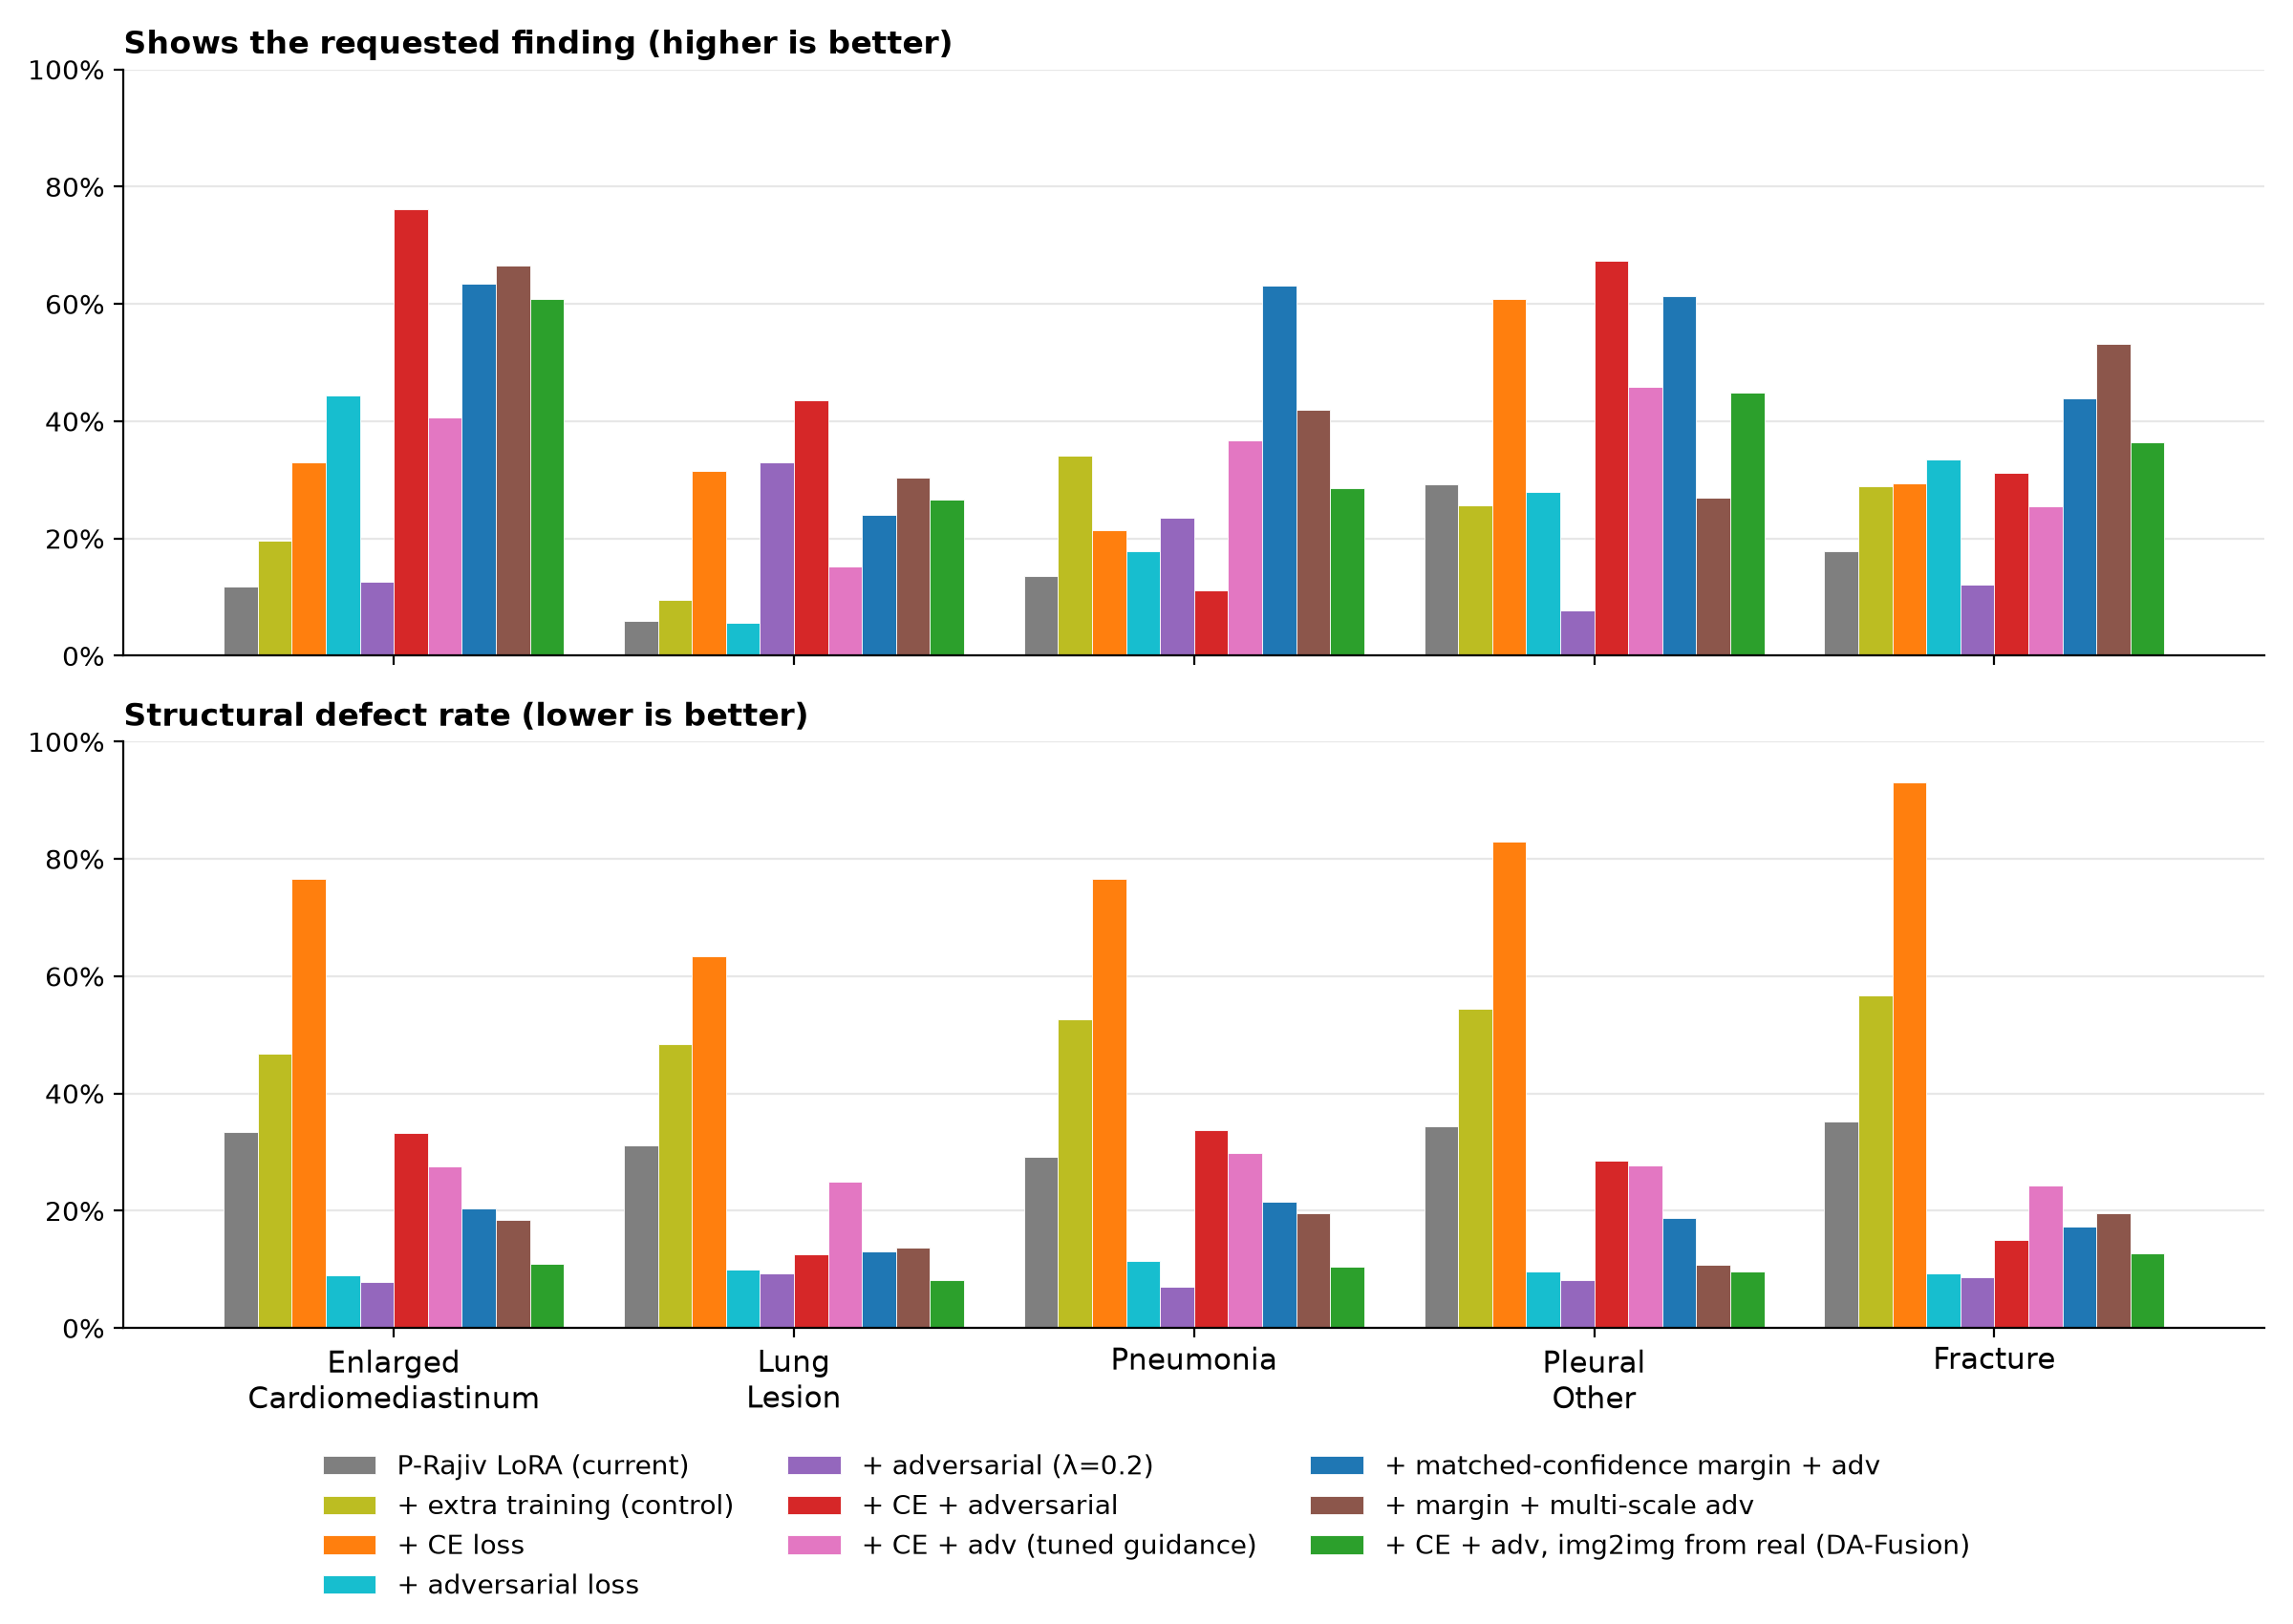
\includegraphics[width=0.93\textwidth]{figs/fig_generation_per_pathology.png}
\caption{Per-pathology requested-finding rate (top) and structural defect rate (bottom) for every generator, scored by the held-out judges.}\label{fig:perpath}
\end{figure}

\begin{figure}[!htbp]
\centering
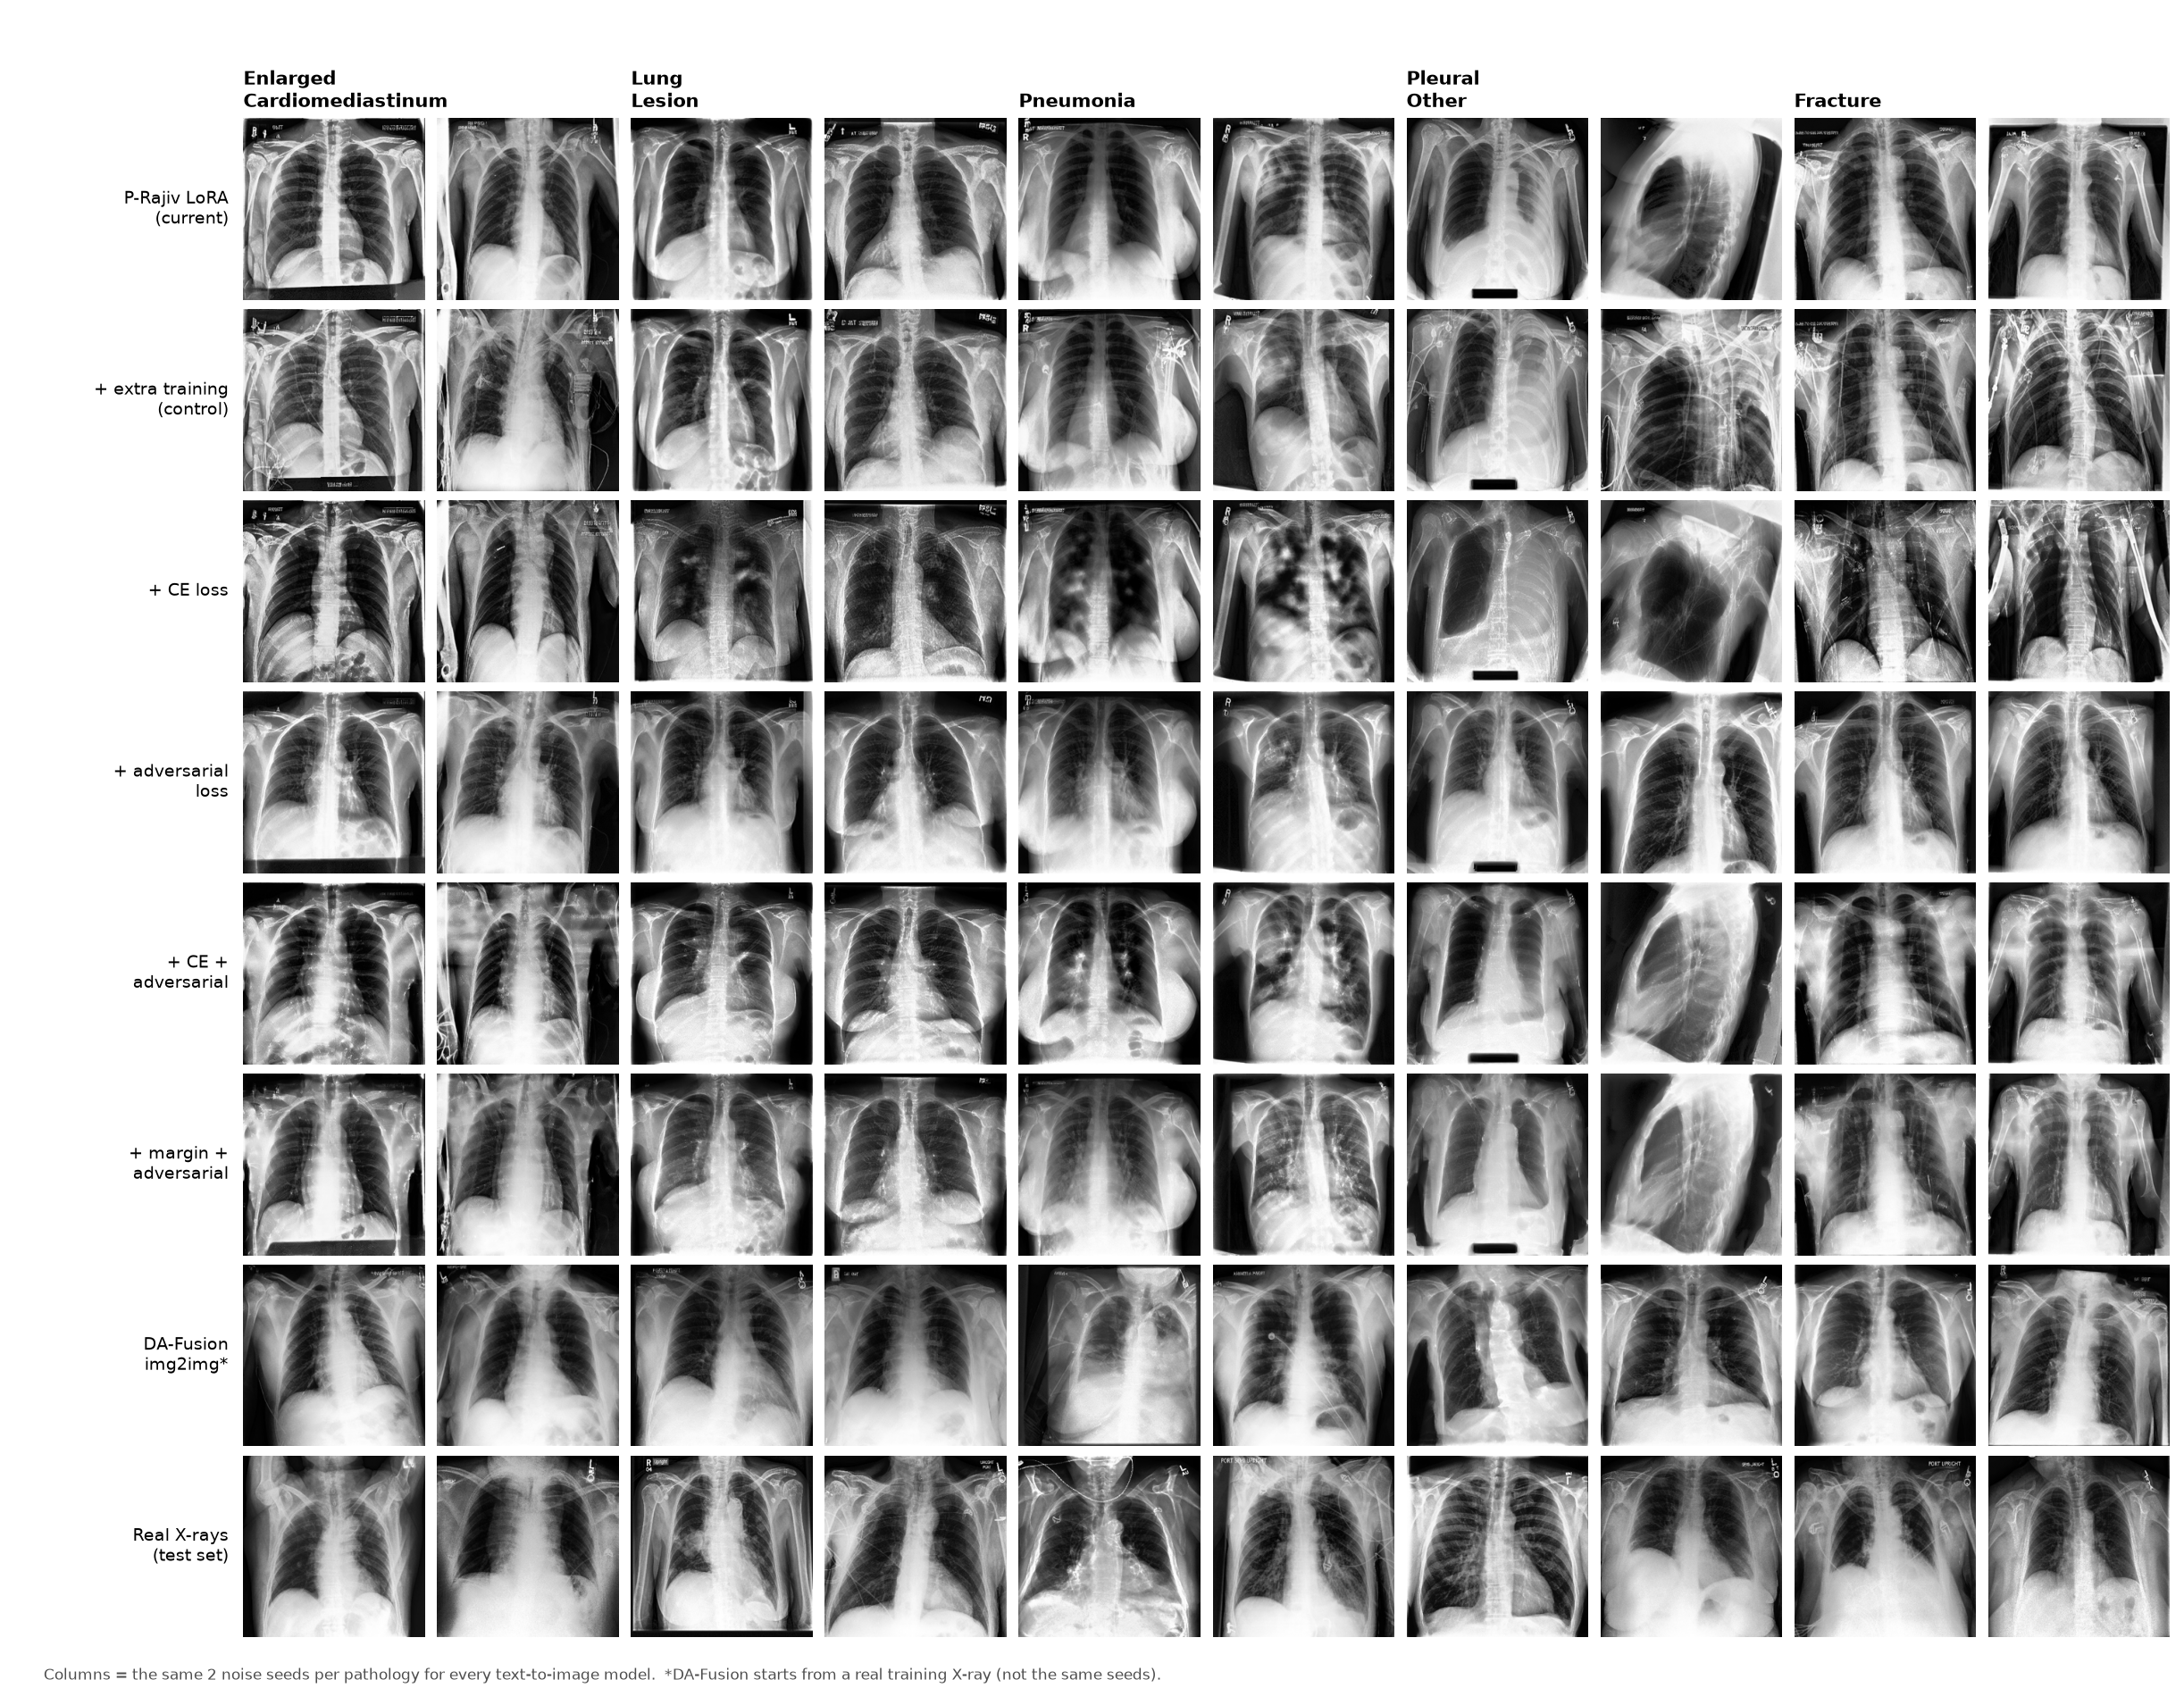
\includegraphics[width=0.93\textwidth]{figs/fig_samples_same_seeds.png}
\caption{Samples from every generator with the \emph{same} two noise seeds per pathology (DA-Fusion starts from real images). CE-only produces blotchy ``cotton-ball'' textures (reward hacking); adversarial-only images are clean but generic; margin\,+\,adversarial shows findings while keeping anatomy.}\label{fig:samples}
\end{figure}

\textbf{Inferences.}
\begin{itemize}\setlength\itemsep{0pt}
\item \textbf{Only the combination improves both axes.} Margin\,+\,adv raises the requested-finding rate $3.3\times$ (15.7$\to$51.2\%) while reducing defects (32.7$\to$18.2\%) and KID (12.8$\to$7.8). The baseline classifies about half its images as No Finding regardless of the prompt; CE\,+\,adv cuts that to under 10\%.
\item \textbf{The classifier loss alone reward-hacks.} CE-only's held-out defect rate rose from 44\% to 87\% in 1{,}000 steps (93\% on Fracture, 83\% on Pleural Other) with KID 29.9: it adds textures the reward classifier likes. The adversarial term is what keeps images on the real-image manifold.
\item \textbf{Realism alone does not give conditioning.} Adversarial-only is the most realistic (9.8\% defects, KID 2.9) but follows the prompt only 25.9\% of the time; $\lambda_{\text{adv}}=0.2$ makes conditioning \emph{worse} (17.8\%) and reduces diversity, so 0.05 was not too weak.
\item \textbf{The control matters.} 2{,}000 extra steps with $L_{\text{diff}}$ alone \emph{increase} defects to 51.8\%, so the gains are due to the new losses, not to more training.
\item \textbf{Exaggeration caveat.} Normalised conditioning $>1$ (1.57--1.87) means combined-loss images are \emph{more} recognisable than real X-rays (``textbook'' findings). Tuned guidance reduces this to 1.19 and KID to 2.7, at the cost of fewer clear findings. No generator memorises: median nearest-neighbour distance 0.07--0.09 for all.
\item \textbf{Multi-scale discriminator: a trade-off, not a win.} Patch heads on three DenseNet stages lowered defects (18.2$\to$16.5\%) and OOD rate (12.9$\to$11.8\%) and brought normalised conditioning closer to real (1.87$\to$1.57, less exaggeration), but the requested-finding rate fell (51.2$\to$43.8\%) and KID rose slightly (7.8$\to$8.7). Its held-out score peaked earlier (step 1{,}000) and then degraded, as in the other CE-based runs.
\item \textbf{Checkpoint selection matters} (Fig.~\ref{fig:ckpt}): CE-based runs peak at step 1{,}000--1{,}500 and then degrade (CE+adv defects 27\%$\to$42\% by step 2{,}000; margin+adv findings 57\%$\to$40\%).
\end{itemize}

\begin{figure}[!htbp]
\centering
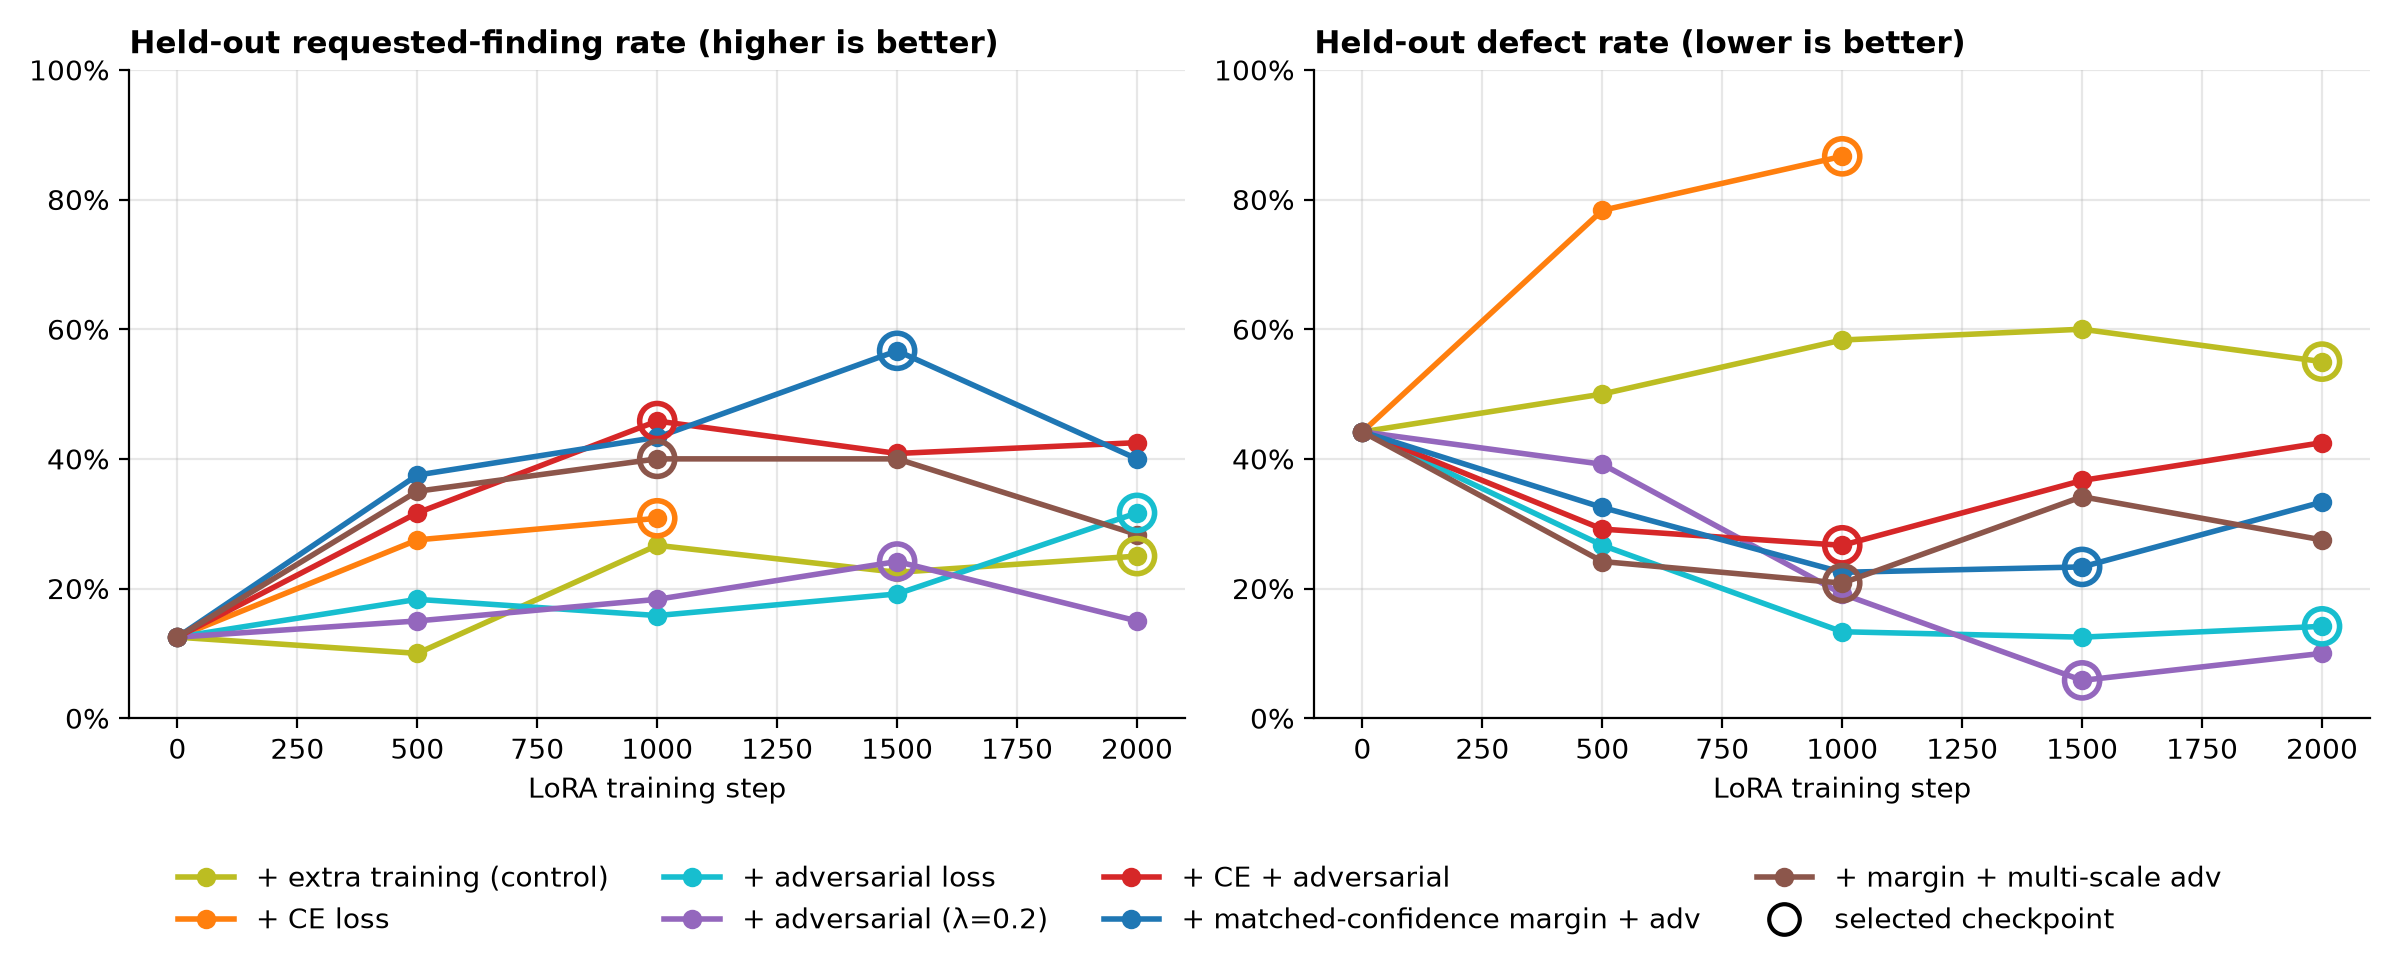
\includegraphics[width=0.85\textwidth]{figs/fig_checkpoint_selection.png}
\caption{Held-out requested-finding rate (left) and defect rate (right) on the fixed seed grid along LoRA training; circles mark the selected checkpoints. Loss curves would not reveal the mid-training peak of the CE-based runs.}\label{fig:ckpt}
\end{figure}

\subsection{Downstream classifier}
\begin{table}[!htbp]
\centering\small
\caption{Test macro-F1 of the 14-class DenseNet-121 (700 real test images, mean $\pm$ std over 3 seeds, epoch selected on validation). [recipe] = real-count class weights, synthetic weight 0.5, last 3 epochs real-only.}\label{tab:ds}
\resizebox{\linewidth}{!}{%
\begin{tabular}{@{}lc@{\hspace{8mm}}lc@{}}
\toprule
Setting & Macro-F1 & Setting & Macro-F1\\
\midrule
\textbf{Real only} & \textbf{0.285$\pm$0.012} & Real + CE+Adv [recipe] & 0.283$\pm$0.015\\
Real + P-Rajiv (baseline) & 0.256$\pm$0.013 & Real + CE+Adv [recipe + filter] & 0.270$\pm$0.024\\
Real + control & 0.275$\pm$0.011 & Real + Margin+Adv [recipe] & 0.279$\pm$0.007\\
Real + CE only & 0.258$\pm$0.017 & Real + CE+Adv tuned guidance [recipe] & 0.272$\pm$0.016\\
Real + Adv only & 0.270$\pm$0.019 & Real + DA-Fusion & 0.253$\pm$0.016\\
Real + Adv only ($\lambda=0.2$) & 0.251$\pm$0.009 & Real + DA-Fusion [recipe] & 0.255$\pm$0.007\\
Real + CE+Adv & 0.269$\pm$0.004 & Real + DA-Fusion [recipe + filter] & 0.279$\pm$0.012\\
Real + CE+Adv, CheXpert-style + NF & 0.254$\pm$0.017 & Real + Margin+Adv multi-scale $D$ & 0.264$\pm$0.010\\
Real + CE+Adv, tuned guidance & 0.256$\pm$0.014 & Real + Margin+Adv multi-scale $D$ [recipe] & 0.281$\pm$0.019\\
Real + Margin+Adv & 0.278$\pm$0.008 & & \\
\bottomrule
\end{tabular}}
\end{table}

\begin{table}[!htbp]
\centering\small
\caption{Per-pathology test F1 for the five generated classes (mean of 3 seeds).}\label{tab:dsper}
\resizebox{\linewidth}{!}{%
\begin{tabular}{@{}lcccccc@{}}
\toprule
Setting & Enl.\ Cardiomed. & Lung Lesion & Pneumonia & Pleural Other & Fracture & Mean of 5\\
\midrule
Real only & \textbf{0.311} & \textbf{0.264} & 0.204 & 0.198 & 0.286 & \textbf{0.253}\\
+ P-Rajiv (baseline) & 0.237 & 0.210 & 0.102 & 0.112 & 0.287 & 0.190\\
+ CE+Adv [recipe] & 0.236 & 0.217 & 0.233 & 0.134 & 0.334 & 0.231\\
+ Margin+Adv [recipe] & 0.281 & 0.256 & 0.207 & 0.154 & \textbf{0.342} & 0.248\\
+ Margin+Adv multi-scale $D$ [recipe] & 0.277 & 0.237 & \textbf{0.240} & \textbf{0.200} & 0.297 & 0.250\\
+ DA-Fusion [recipe + filter] & 0.239 & 0.262 & 0.223 & 0.152 & 0.284 & 0.232\\
\bottomrule
\end{tabular}}
\end{table}

\begin{figure}[!htbp]
\centering
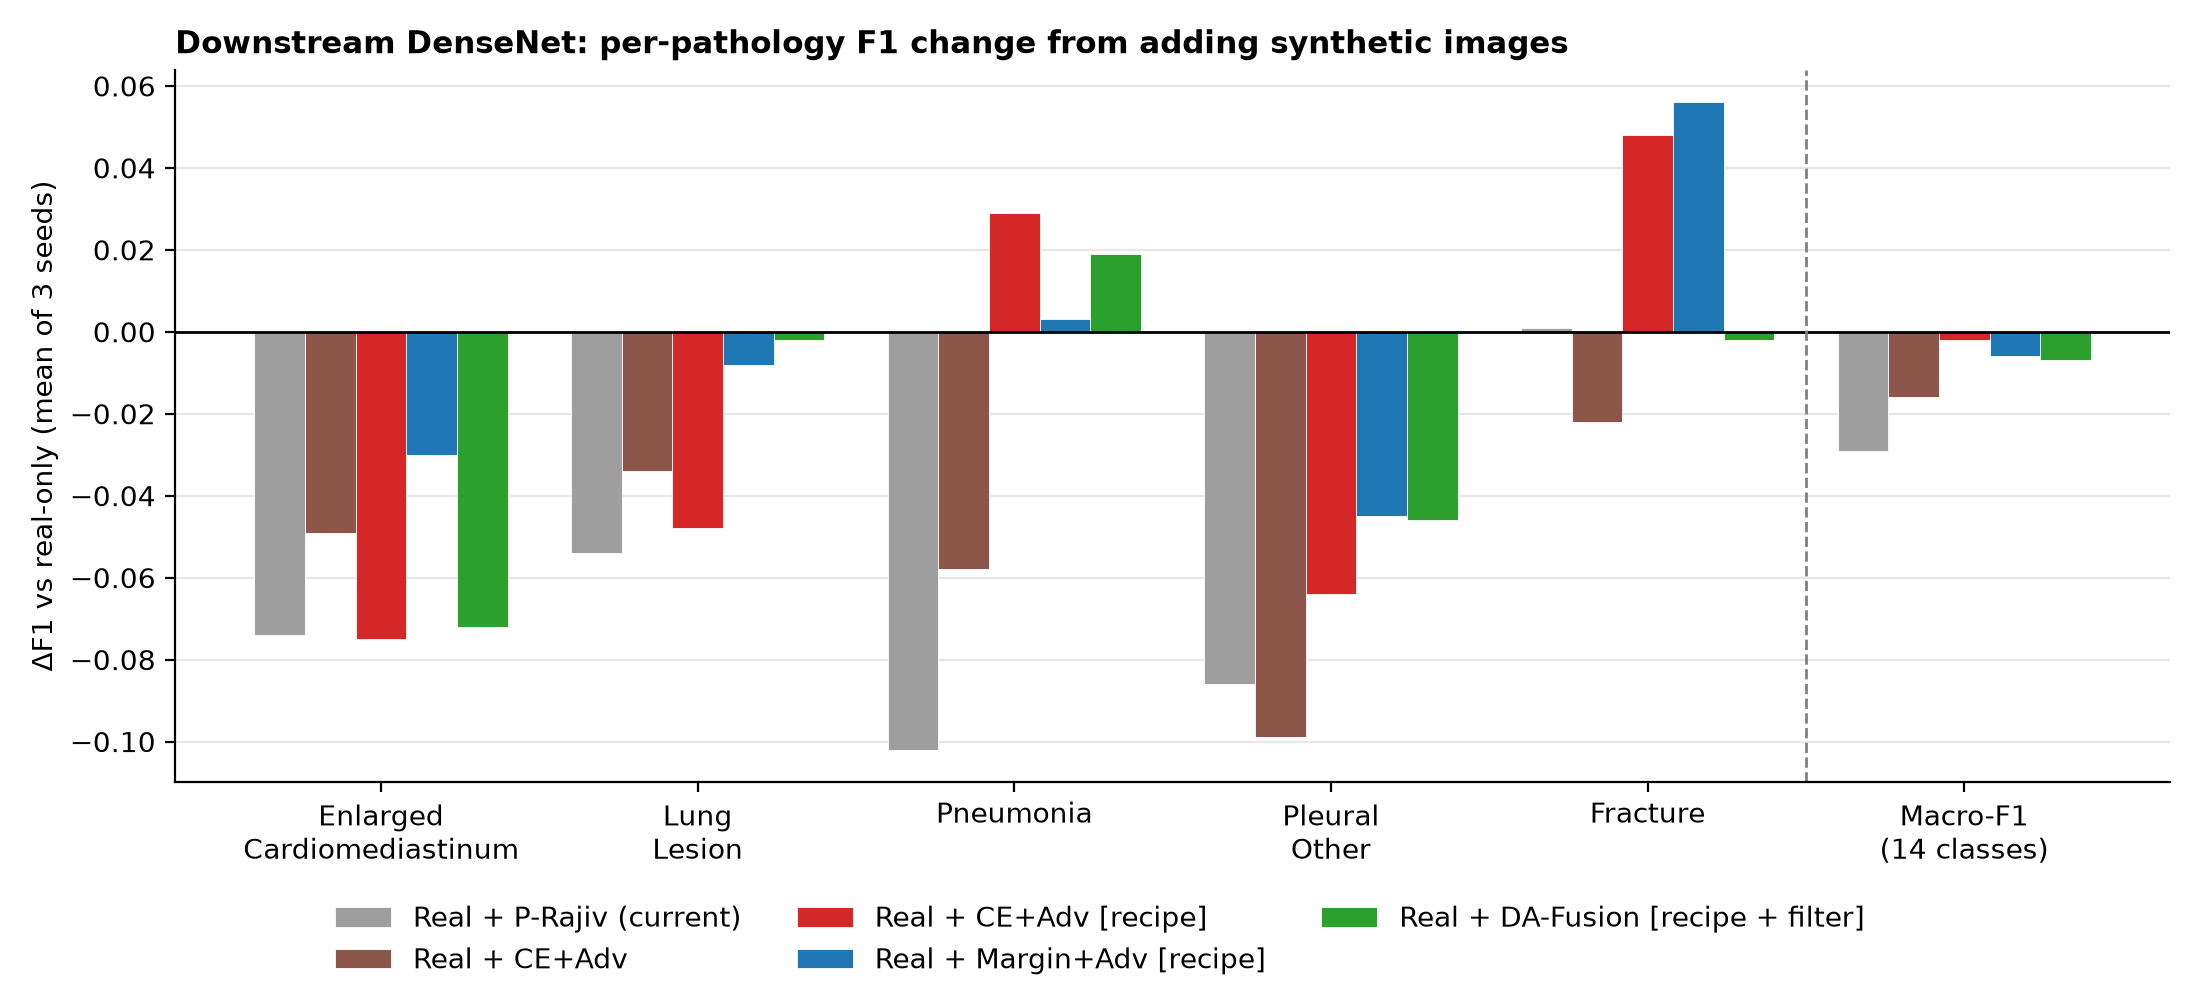
\includegraphics[width=0.85\textwidth]{figs/fig_downstream_delta_key.png}
\caption{Per-pathology change in test F1 relative to real-only training for the key settings.}\label{fig:delta}
\end{figure}

\textbf{Inferences.}
\begin{itemize}\setlength\itemsep{0pt}
\item \textbf{Parity, not improvement.} The original P-Rajiv augmentation lowers macro-F1 (0.285$\to$0.256). With the new generators and the recipe, augmentation reaches parity (CE+Adv [recipe] 0.283$\pm$0.015; Margin+Adv [recipe] 0.279$\pm$0.007, the smallest seed spread). No setting beats real-only; with std $\approx0.012$ over 3 seeds, differences below $\approx0.02$ are within noise. AUROC barely moves (0.763--0.778 across all 19 settings).
\item \textbf{How synthetic data enters training matters as much as its quality.} The recipe lifts CE+Adv from 0.269 to 0.283 and DA-Fusion (best image metrics) from 0.253 to 0.279 (with filtering). Image-quality metrics did not predict downstream usefulness.
\item \textbf{Per pathology:} Fracture improves with both combined-loss generators (+0.048, +0.056); Pneumonia with CE+Adv (+0.029), after the baseline had halved it; Pleural Other (241 real images, subtle findings) gets worse in 17 of 18 synthetic settings ($-0.04$ to $-0.16$); the exception is the multi-scale-$D$ generator with the recipe (0.200 vs.\ 0.198, i.e.\ level), which also gives the largest Pneumonia gain (+0.036) and macro-F1 0.281$\pm$0.019 --- the second-best synthetic setting, within seed noise of real-only. Gains on non-generated classes (e.g.\ Consolidation +0.051) offset these losses.
\end{itemize}

\subsection{Why real + synthetic does not beat real-only in our setting}\label{sec:whynot}
Parity rather than improvement is what the literature predicts for our regime. The reported gains from generated training data come from conditions our setup does not meet:
\begin{itemize}\setlength\itemsep{0pt}
\item \textbf{Full-data, in-distribution regime.} Gains concentrate where real data is scarce and shrink as it grows. He et al.\ restrict their classification study to zero- and few-shot settings because the positive impact of synthetic data diminishes as more real shots are present~\citep{he2023synthetic}. RoentGen's AUROC gain (+0.04) is for a small real set~\citep{chambon2022roentgen}. Prakash et al.\ report large pneumonia F1 gains with 1\% of the real data but only marginal gains with 100\%~\citep{prakash2025synthetic}. The clearest medical benefits are for robustness and fairness under distribution shift~\citep{ktena2024fairness}. Our classifier already has 214--1{,}369 real images per class and is tested in-distribution on CheXpert.
\item \textbf{No information beyond the real training set.} Our LoRA is fine-tuned on CheXpert training images with the same labeler-derived labels the classifier sees. It can re-sample that data but cannot add knowledge about $p(y\mid x)$. Successful cases use a generator trained on more or different data: RoentGen on MIMIC-CXR~\citep{chambon2022roentgen}, or Imagen fine-tuned on ImageNet and sampled at up to $3\times$ the real-set size~\citep{azizi2023synthetic}. Khosravi et al., with diffusion models trained on CheXpert, MIMIC-CXR and Emory data, conclude that real data remains superior~\citep{khosravi2024synthetically}. Ravuri and Vinyals find that adding BigGAN samples to the full ImageNet training set improves accuracy at most marginally~\citep{ravuri2019cas}.
\item \textbf{Image metrics do not predict usefulness.} IS and FID are not predictive of a generator's classification accuracy score~\citep{ravuri2019cas}, and our metrics behave the same way. CE+Adv shows the requested Enlarged Cardiomediastinum finding in 76\% of images, yet Enlarged Cardiomediastinum F1 falls from 0.311 to 0.236. A normalised conditioning of 1.87 (Margin+Adv) means the probe finds the synthetic images \emph{easier} than real ones. They are prototypical examples that add little near the decision boundary, which is where real errors occur.
\item \textbf{Label noise caps the task.} Even on real images, the held-out probe reaches only 29.7\% (chance 16.7\%), and the real-only DenseNet reaches 29.6\% accuracy on the balanced 14-class test set. Rare-class errors are mostly confusions with No Finding and Fracture, which synthetic images of the rare class cannot resolve. With Margin+Adv [recipe], more Pleural Other test images are predicted as No Finding (9.7$\to$15.7 of 50, averaged over seeds).
\item \textbf{Scale and statistical power.} 2{,}173 synthetic images ($\approx$13\% of the training set) affect only 5 of the 14 classes. With 50 test images per class and 3 seeds, differences below $\approx$0.02--0.03 macro-F1 cannot be resolved.
\end{itemize}
The settings where gains are expected --- scarce real data and shifted test distributions --- are therefore the natural next experiments (Sec.~\ref{sec:Plan for Novelty Assessment}).

\textbf{Limitations.} 50 test images per class makes per-class F1 noisy (0.05 $\approx$ 2--3 images); metrics come from classifiers, not radiologists; reward and evaluator share the DenseNet-121 architecture; only six template prompts; each LoRA variant trained with one seed.

%======================================================================
\section{Ongoing and Future Work}\label{sec:Plan for Novelty Assessment}
\begin{enumerate}\setlength\itemsep{0pt}
\item \textbf{Regimes where synthetic data is expected to help} (Sec.~\ref{sec:whynot}): a low-data study that keeps only 10--25\% of the real rare-class images~\citep{prakash2025synthetic}, and evaluation on a shifted test set from another hospital, e.g.\ MIMIC-CXR or NIH ChestX-ray14~\citep{ktena2024fairness}.
\item \textbf{Discriminator design:} the multi-scale $D$ (Sec.~\ref{sec:ms}) traded conditioning for realism; re-balancing $\lambda_{\text{cls}}$ against the stronger $D$, or per-scale weights, is the next step.
\item \textbf{Multi-step reward gradients} (DRaFT-$K$~\citep{clark2024draft}) instead of the one-step estimate, and a KL penalty to the base model~\citep{fan2023dpok} as a principled anti-hacking term.
\item \textbf{Report-level prompts} from CheXpert Plus~\citep{chambon2024chexpertplus} to control location and severity.
\item \textbf{Reward usefulness directly:} score synthetic batches by the improvement they give a classifier on held-out real data; per-class choice of $\lambda_{\text{cls}}$, guidance and number of synthetic images (keep Fracture gains, avoid Pleural Other losses).
\item \textbf{Validation of metrics} by a radiologist; larger test set and more seeds to make $\approx0.03$ F1 differences testable.
\end{enumerate}

%======================================================================
\section{Conclusion}\label{sec:conclusion}
We studied whether a LoRA-fine-tuned text-to-image diffusion model can generate useful rare-pathology chest X-rays. The standard denoising loss alone produced images that mostly ignored the prompt. Adding a frozen-classifier loss and a class-conditional projection-discriminator loss, both on a differentiable one-step estimate of the generated image, tripled the rate at which images show the requested finding while reducing structural defects and KID, as judged by held-out models. The classifier signal alone reward-hacks; a bounded, real-matched margin loss plus the adversarial regulariser controls this. Downstream, the improved generators and a corrected training recipe turn a harmful augmentation into one at parity with real-only training, with consistent gains on Fracture, but not an overall improvement --- consistent with prior findings that synthetic data helps mainly when real data is scarce or the test distribution is shifted, and that real data remains superior in the full-data, in-distribution regime (Sec.~\ref{sec:whynot}). Better image metrics did not automatically translate into a better classifier, which motivates rewarding downstream usefulness directly in future work.

\bibliographystyle{plain}
\bibliography{refs}

\end{document}
